%% ------------------------------------------------------------------------- %%
\chapter{Fossil Fishes from the Sincejelo and Ware formations}
\label{chap:chapFossilFishes}

\section{Introdução}

Lorem ipsum dolor sit amet, consectetur adipiscing elit. Nam vel vestibulum sapien. Suspendisse tempus arcu eu porttitor dignissim. Duis eget sapien tempus, facilisis ligula sed, euismod quam. Quisque ultricies non purus vestibulum efficitur. Sed ut libero mauris. Donec ultricies nisi vitae luctus volutpat. Mauris pretium lacinia velit et luctus. Vivamus id augue a purus varius sagittis. Aenean aliquet lectus sed condimentum posuere. Sed pharetra lacinia consectetur. Curabitur viverra ultrices enim, id hendrerit est egestas vitae. Nunc euismod, enim aliquet fermentum mollis, enim sem ornare nisi, vitae volutpat arcu tortor et orci. Proin tellus nunc, vehicula at est quis, maximus fringilla mi \citep{Nascimento2005,Nascimento2006}.

\subsection{Sub-topico da introdução}

Donec ut ligula leo. Suspendisse ultrices tempor pharetra. Vivamus arcu lacus, vulputate at risus in, vestibulum tristique eros. Etiam consectetur id leo ut viverra. Aliquam viverra elit sit amet eros bibendum, ac mollis quam posuere. Pellentesque risus odio, molestie tempus fermentum vitae, egestas eget massa. Mauris eu risus quis leo accumsan rhoncus. Suspendisse rhoncus justo a purus elementum, at scelerisque tellus auctor. Nullam suscipit eleifend dignissim. Maecenas at erat tellus.

\subsection{Um outro subtopico da introdução}

Integer consequat, odio pharetra condimentum maximus, lacus sem tincidunt est, vitae cursus diam velit vitae turpis. Proin cursus varius nibh, in suscipit velit eleifend et. Cras vel lobortis felis. Pellentesque habitant morbi tristique senectus et netus et malesuada fames ac turpis egestas. Nam vitae mauris scelerisque, volutpat leo iaculis, congue enim. Nam vehicula, lorem sagittis hendrerit iaculis, risus erat cursus lacus, id hendrerit velit ante id sem. In hac habitasse platea dictumst. Praesent ut nunc maximus, dapibus justo vel, commodo tortor. Quisque vel feugiat ipsum, a ultricies mauris. Nulla id lacinia ex. Proin dignissim nisl dictum diam interdum convallis.

\section{Materiais e Métodos}

Os listados podem-se especificar por meio do ambiente itemize

\begin{itemize}
  \item Cras sed odio nec
  \item Maecenas sollicitudin metus vel
  \item Donec faucibus orci ac turpis blandit maximus
\end{itemize}

Cras sed odio nec metus vulputate ultricies in vitae urna. Sed vulputate libero a ante hendrerit pellentesque. Vivamus sem nibh, eleifend non tristique sit amet, vestibulum quis lorem. Donec in ipsum rhoncus turpis tincidunt luctus. Proin nec egestas ipsum, quis varius ipsum. Suspendisse consectetur sagittis est, vel dapibus dolor laoreet at. Maecenas sollicitudin metus vel ornare malesuada. Maecenas rhoncus molestie est, quis cursus dui suscipit vel. Quisque iaculis aliquam arcu, ut pharetra nulla rhoncus id. Fusce et lacus eget arcu sodales volutpat. Duis quis turpis sit amet mauris laoreet fermentum. Sed et nunc finibus arcu interdum scelerisque.

As figuras, por meio do ambiente figure (e.g., La Figura \ref{fig:dorsal}) e a função includegraphics.

\begin{figure}
\centering
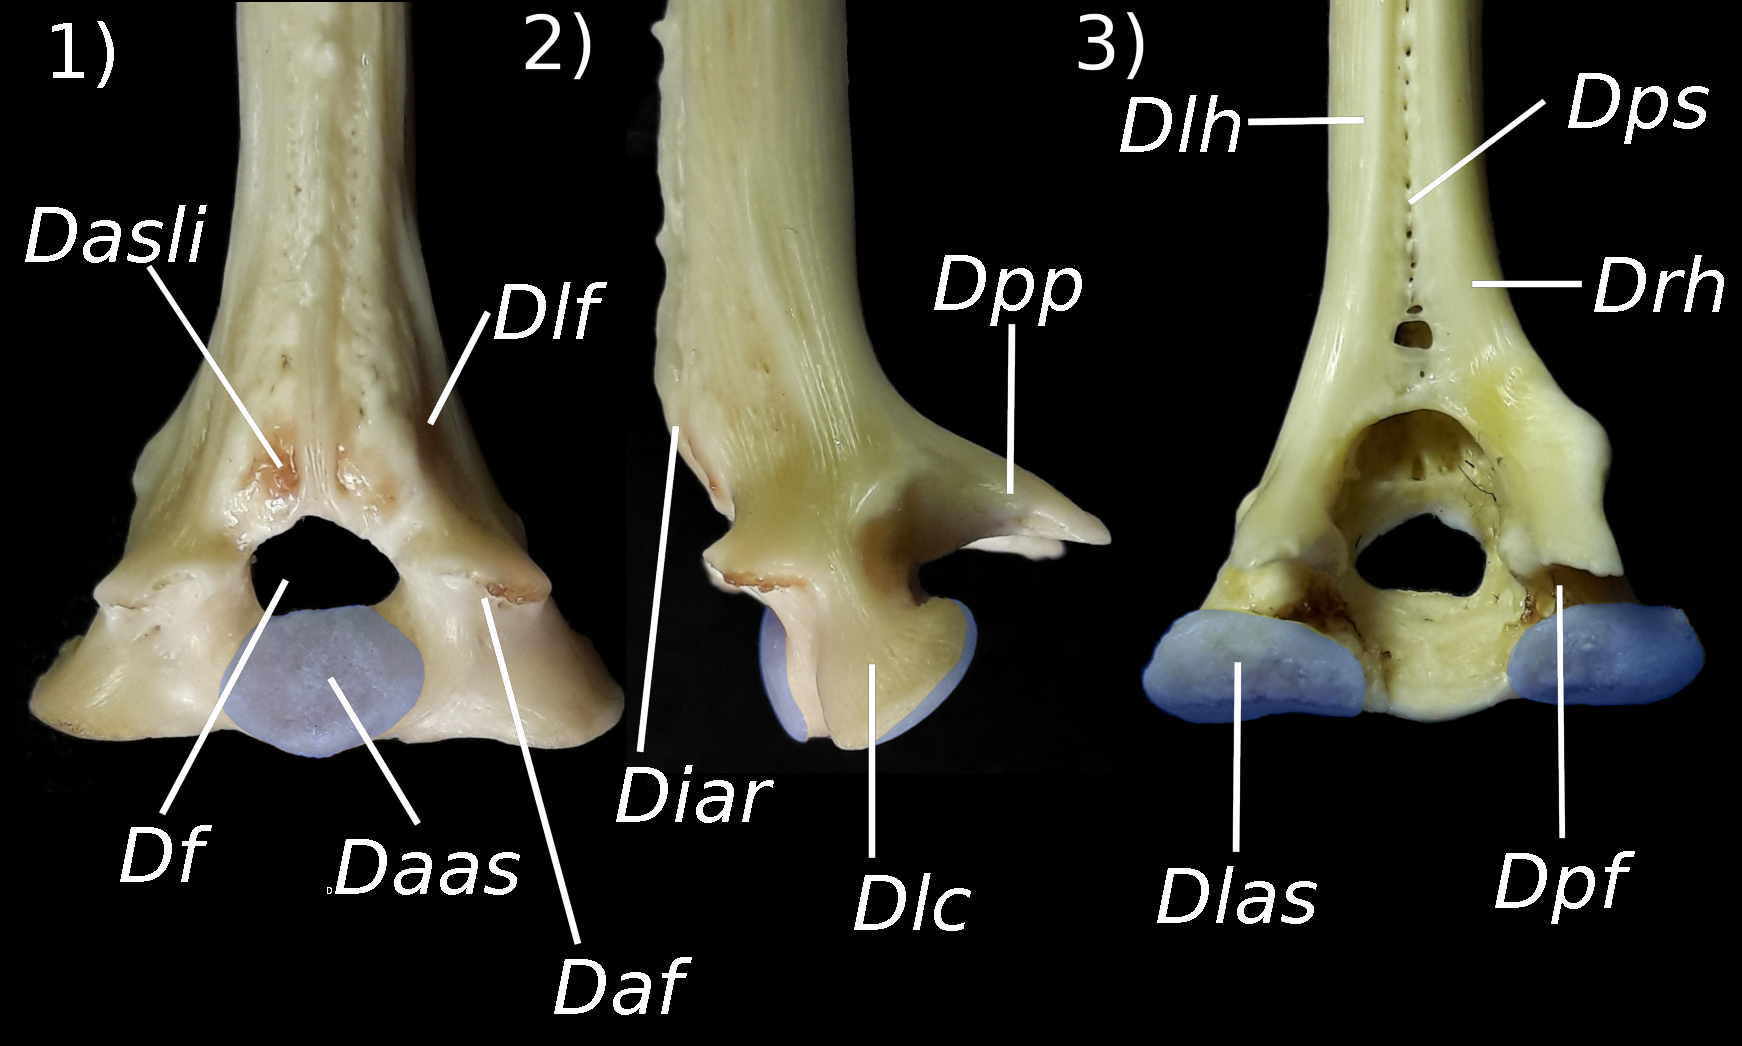
\includegraphics[width=\textwidth]{dorsal}
\caption{Legenda da figura}
\label{fig:dorsal}
\end{figure}

\section{Resultados}

Vivamus aliquet vitae nibh vel blandit. Mauris sed quam vel dui scelerisque pulvinar et in est. Pellentesque dignissim imperdiet libero in tincidunt. Fusce posuere fermentum justo, ac faucibus augue cursus vitae. Ut dictum vulputate metus, ac semper metus volutpat vitae. Morbi est nibh, consectetur vel ante sit amet, imperdiet venenatis quam. Nulla dictum quam eu orci maximus, vel faucibus magna placerat. Nullam libero est, tincidunt bibendum condimentum sed, rhoncus sit amet nulla. Vestibulum at mauris lobortis, malesuada leo in, viverra justo. Aliquam iaculis laoreet est vel faucibus. Donec faucibus orci ac turpis blandit maximus. Nulla semper laoreet lorem, ultrices pulvinar sem tristique eu. Vivamus vel cursus felis, sit amet euismod arcu. Sed sit amet ipsum volutpat, eleifend erat ut, vehicula nulla. Sed viverra nisi sollicitudin, elementum elit sed, suscipit leo. Nulla pulvinar metus at malesuada pretium. 

\section{Discusão}

As tabelas tem uma sintaxe particular, como na Tabela \ref{tab:tabelaExemplos}

\begin{table}
\begin{center}
\caption{O titulo das tabelas geralmente debe se posicionar encima da tabela} \label{tab:tabelaExemplos}
    \begin{tabular}{ | l | l | l | p{5cm} |}
    \hline
    Day & Min Temp & Max Temp & Summary \\ \hline
    Monday & 11C & 22C & A clear day with lots of sunshine.  
    However, the strong breeze will bring down the temperatures. \\ \hline
    Tuesday & 9C & 19C & Cloudy with rain, across many northern regions. Clear spells 
    across most of Scotland and Northern Ireland, 
    but rain reaching the far northwest. \\ \hline
    Wednesday & 10C & 21C & Rain will still linger for the morning. 
    Conditions will improve by early afternoon and continue 
    throughout the evening. \\
    \hline
    \end{tabular}
\end{center}
\end{table}

\bibliographystyle{palelec} % citação bibliográfica segundo o formato da revista Palaeontologia Electronica
\bibliography{refs/BiblioTese}  % associado ao arquivo: BiblioTese.bib'